%!TEX root = ../report.tex

\chapter{State of The Art} \label{chap:chap2}

\section*{}

% TODO dimensions on user experience

\section{Introduction}

In this chapter, the most relevant web services for this thesis will be analysed.

The proposed methodology focus on how the content is presented and less on what the content is (without discarding its importance).
Even so, some projects that focus on the content will be analysed.

The presented projects often use external data bases (like last.fm) to fetch metadata from.
This is the preferred way, since those are the most complete sets of information. 

\section{Related and Similar Services} % (fold)
\label{sec:related_similar_services}

\subsection{Liveplasma - liveplasma.com} % (fold)
\label{sub:liveplasma}

liveplasma.com is a \emph{flash}\footnote{\url{http://get.adobe.com/flashplayer}} application that not only it allows to see a graph of music artists, but also of books and movies.

The interaction with the graph is very faulted: no changes to the graph are allowed, and the user can easily make a mistake and perform unwanted actions like redrawing the graph with another artist as the root node.

\begin{figure}
  \begin{center}
    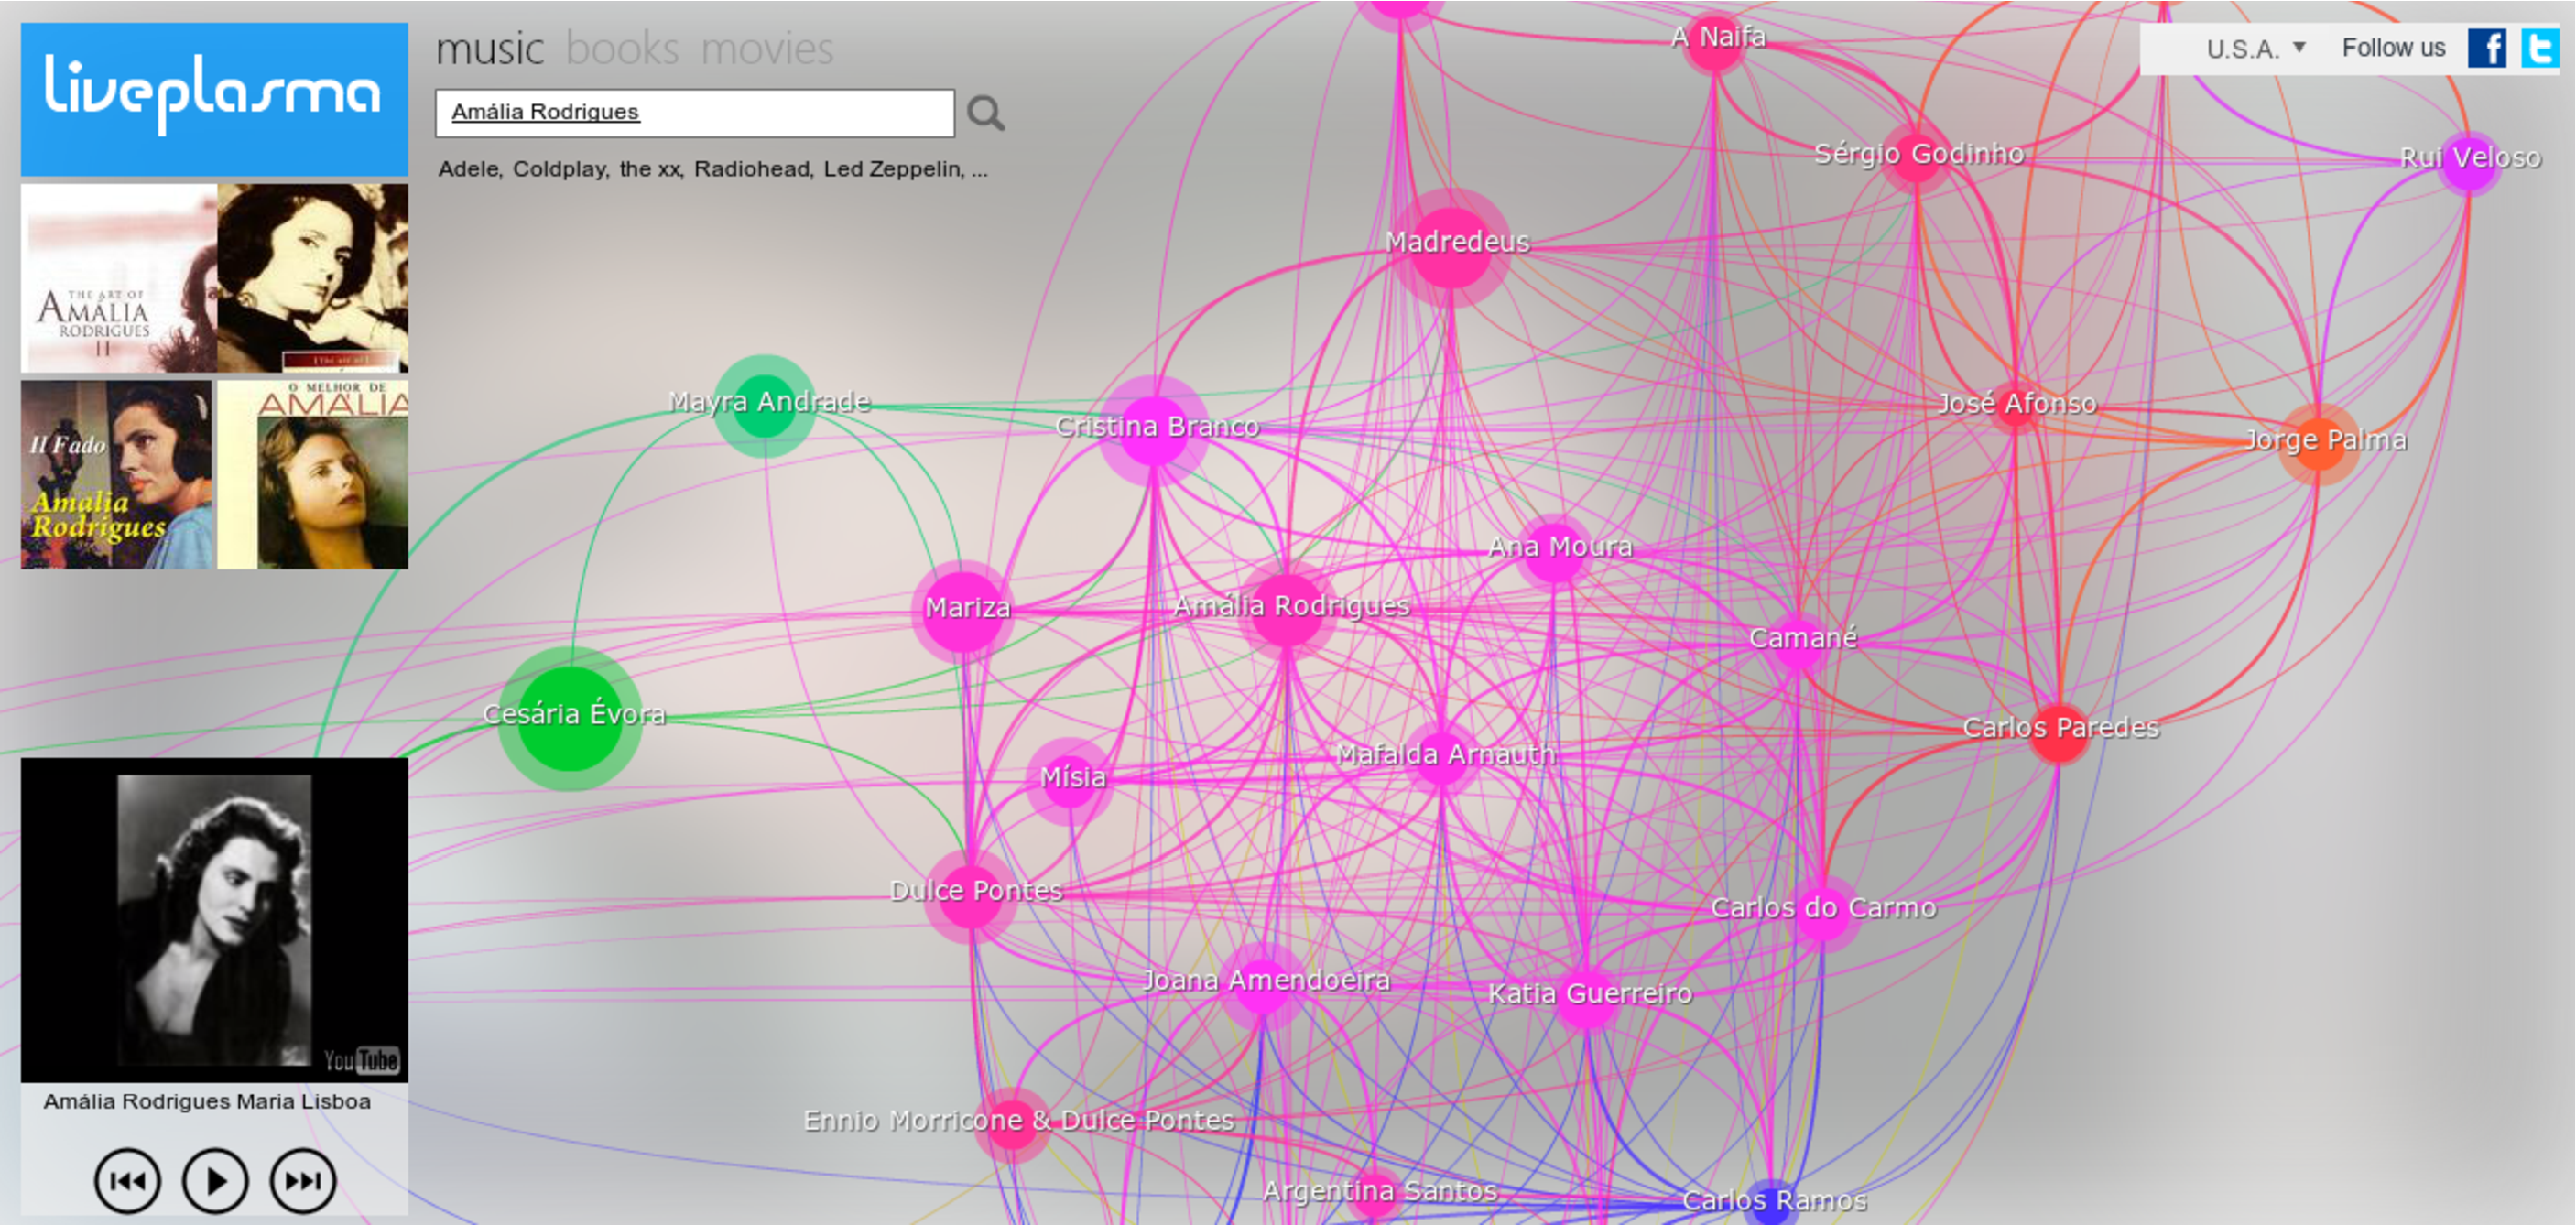
\includegraphics[width=\textwidth]{liveplasma.pdf}
  \end{center}
  \caption{liveplasma: search result for "Amália Rodrigues"; upper left corner: artist albums; lower left corner: youtube's \emph{mini-player}}
  \label{fig:sota_liveplasma}
\end{figure}

In \ref{fig:sota_liveplasma} one can see the search result for "Amália Rodrigues".

On the left side of the application there are some interesting elements: a grid of the artist's albums, a mini-player (stream from Youtube).

In \ref{fig:sota_liveplasma2} the user can have the choice to play tracks \emph{only} from that artist, or play \emph{similar} artists.

\begin{figure}[b]
  \begin{center}
    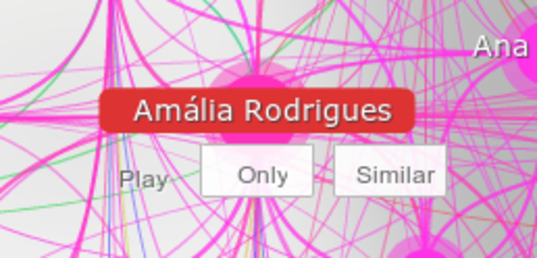
\includegraphics[]{liveplasma2.pdf}
  \end{center}
  \caption{liveplasma: interface to start playing tracks. \emph{Similar} button plays tracks from similar artists, whereas, the \emph{only} button only plays tracks from the specified artist.}
  \label{fig:sota_liveplasma2}
\end{figure}

\subsubsection{Pros} % (fold)
\label{ssub:liveplasma_pros}

This tools, has two interesting aspects to it:

\begin{itemize}
  \item Links to buy albums of the artist
  \item Play tracks from similar artists to the search artist.
\end{itemize}

% subsubsection pros (end)

\subsubsection{Cons} % (fold)
\label{ssub:liveplasma_cons}

The graph drawn from this simple search, is very cluttered with edges.
Two nodes can have several connections between, which seems to overload the graph and making it very confusing.

Different colours are used, but their meaning remains unknown. One can assume that they represent the similarity between artists, but that is just speculation.

It can also be assumed that the size of the nodes (radius value) can be directly proportional to the artist's popularity, but that is, again, just speculation.

One critical detail is that the user cannot visually point out the search node in the graph, given the lack of visual distinction from the other nodes of the graph \ref{fig:sota_liveplasma}.


% subsubsection cons (end)

\subsubsection{Summary} % (fold)
\label{ssub:liveplasma_summary}

In short, liveplasma is not very user friendly. 
It uses too many colours and edges, which makes the user experience of searching for new music even harder than usual.

% subsubsection summary (end)

% subsection liveplasma (end)

\subsection{Tuneglue - audiomap.tuneglue.net} % (fold)
\label{sub:tuneglue}

Tuneglue is another flash application that tries to explore the graphic visualization of network of related artists.
Last.fm's metadata API is used to retrieve artist information.

When you start Tuneglue and search for an artist, say "Mariza", the user is presented with a single-node graph.
By clicking the node, the user has four options (\ref{fig:sota_tuneglue}): expand, releases, lock position and delete.


\begin{figure}[bt]
  \begin{center}
    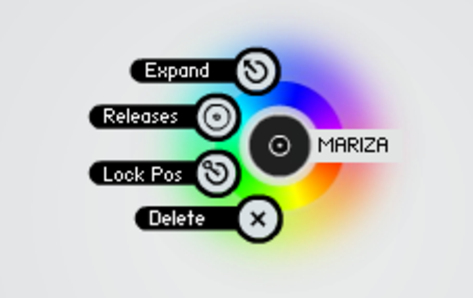
\includegraphics[]{tuneglue.pdf}
  \end{center}
  \caption{Tuneglue: menu for the node. Appears when the user clicks the node.}
  \label{fig:sota_tuneglue}
\end{figure}

When you first expand a node, you get the root node with six child nodes \ref{fig:sota_tuneglue2}.

\begin{figure}[tb]
  \begin{center}
    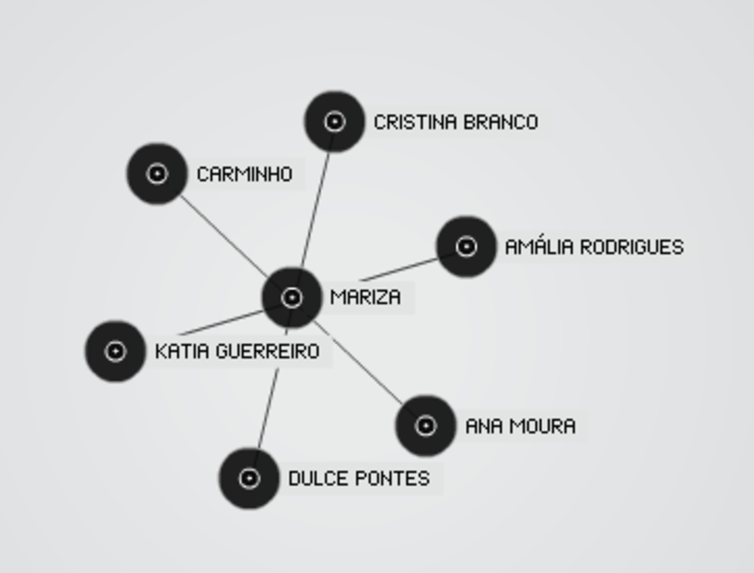
\includegraphics[]{tuneglue2.pdf}
  \end{center}
  \caption{Tuneglue: graph after expanding the root node.}
  \label{fig:sota_tuneglue2}
\end{figure}

So the first feature that brings the user experience to another level (in comparison with liveplasma) is that of graph editing.
The user can expand, fix and delete every single node in the graph.


\subsubsection{Pros} % (fold)
\label{ssub:audiomap_pros}

Tuneglue gives control to the user.
On one hand, the user is able to craft a graph and tailor it to its needs.
The user feels that graph is its own creation.

% subsubsection pros (end)

\subsubsection{Cons} % (fold)
\label{ssub:audiomap_cons}

On the other hand, the user has the responsibility to create the whole graph, which might be too much trouble and deteriorate the user experience.

Again the root node is not highlighted, which might leave the user lost when the graph gets more and more complex.

% subsubsection contras (end)

\subsubsection{Summary} % (fold)
\label{ssub:audiomap_summary}

Tuneglue takes the approach to give the user the power to create what he wants.
But with no limit, the user can easily create a very complex graph that deteriorates the user experience.


% subsubsection summary (end)

% subsection tuneglue (end)

\subsection{MusicRoamer - musicroamer.com} % (fold)
\label{sub:musicroamer}

  MusicRoamer is yet another flash application.
  Although it is similar to Tuneglue when it allows the user to expand the graph further and further, it also imposes some limits to the user to avoid getting the graph confusing.

  \subsubsection{Pros} % (fold)
  \label{ssub:pros}

  There are three types of search \ref{fig:sota_musicroamer}): 

  \begin{description}
    \item[Artist Search] \hfill \\
      The most used one.
    \item[Keyword Search] \hfill \\
      Search using keywords like genres and tags
    \item[Last.fm user search] \hfill \\
      The search result generates several graphs with the top artists of the user as the root nodes.
  \end{description}

  \begin{figure}[tb]
    \begin{center}
      
\includegraphics[width=\textwidth]{musicroamer.pdf}
    \end{center}
    \caption{MusicRoamer: Search options. by artist; by keyword and by Last.fm username}
    \label{fig:sota_musicroamer}
  \end{figure}

  Independently of the search form used, the result will always be one (or more) graphs where the nodes are music artists.

  MusicRoamer is worth mentioning because of the way it shows the graph.
  In \ref{fig:sota_musicroamer2} one can see the search result for "Mariza".

  \begin{figure}[tb]
    \begin{center}
      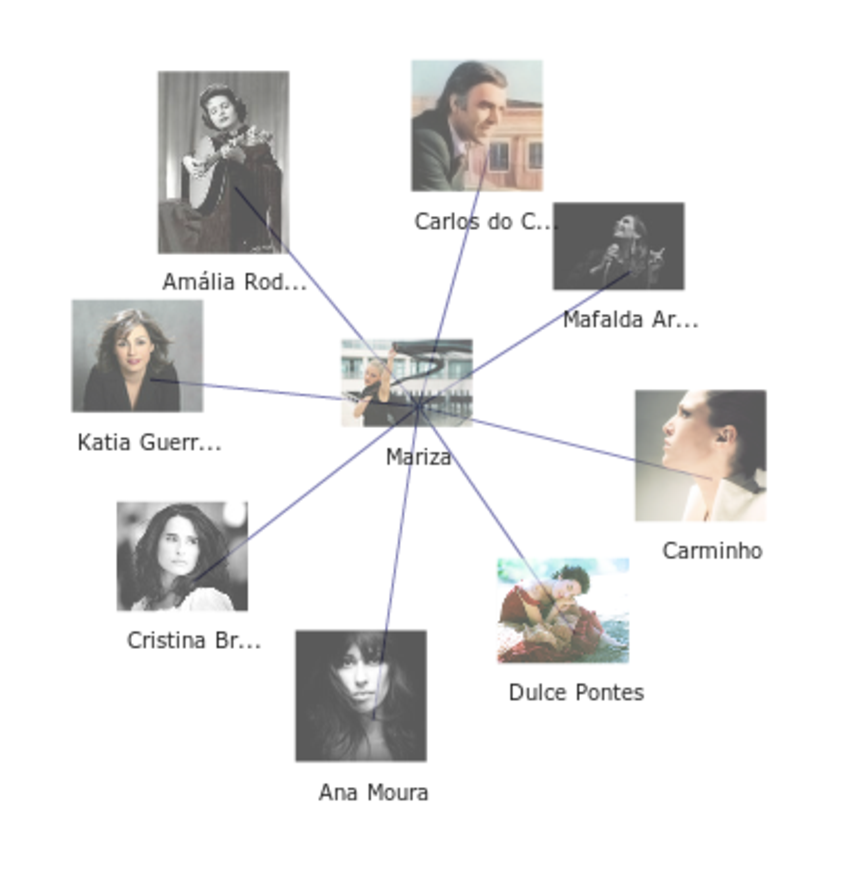
\includegraphics[width=\textwidth]{musicroamer3.pdf}
    \end{center}
    \caption{MusicRoamer: Visual representation of the artist graph}
    \label{fig:sota_musicroamer2}
  \end{figure}

  The images of the music artists are used to represent the nodes. This way, the user has a more friendly mind map of the resulting graph.

  There is also some parameters (\ref{fig:sota_musicroamer3}) that the user can personalize to change the appearance of the graph: zoom; repulsion force between the nodes; size of the artist's images and the number of artist to be used as the branching value.

  \begin{figure}[tb]
    \begin{center}
      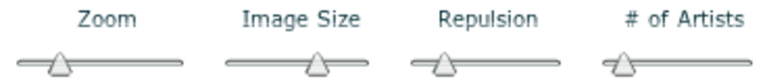
\includegraphics[width=\textwidth]{musicroamer2.pdf}
    \end{center}
    \caption{MusicRoamer: Personalizable parameters for the graph }
    \label{fig:sota_musicroamer3}
  \end{figure}

  % subsubsection pros (end)

  \subsubsection{Cons} % (fold)
  \label{ssub:cons}

  MusicRoamer is a flash application which makes the interface less natural and fluid to a website user.

  Another problem occurs when the user starts to expand more and more nodes.
  The graph starts to get confusing (\ref{fig:sota_musicroamer4}), the edges are drawn over the images, the artist's names start to get mixed in the images.

  \begin{figure}[tb]
    \begin{center}
      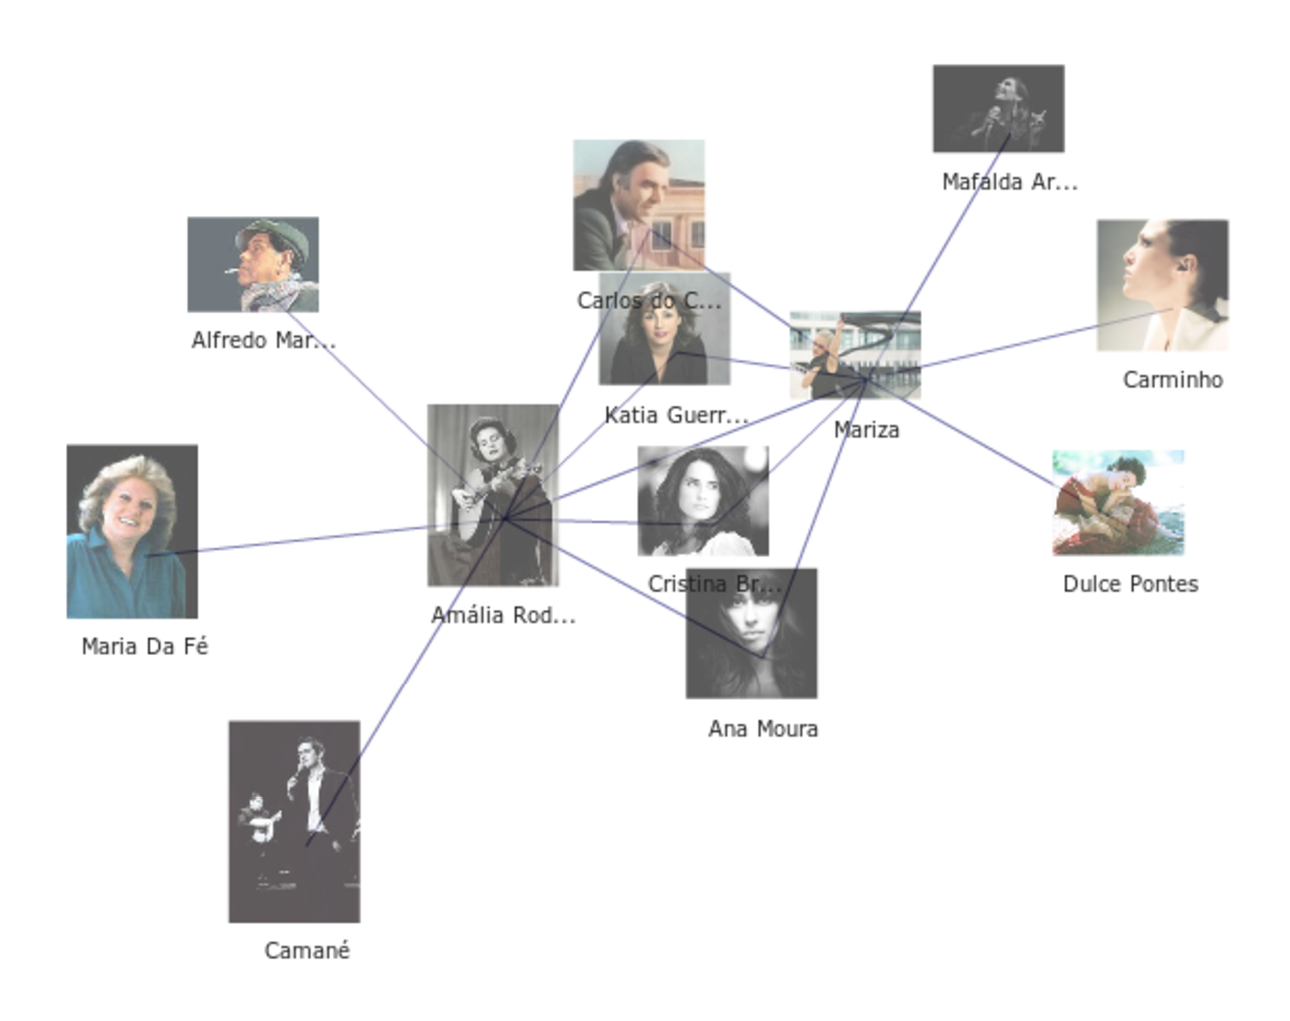
\includegraphics[width=\textwidth]{musicroamer4.pdf}
    \end{center}
    \caption{MusicRoamer: The graph after expanding one node}
    \label{fig:sota_musicroamer4}
  \end{figure}

  % subsubsection cons (end)

  \subsubsection{Summary} % (fold)
  \label{ssub:summary}

  Although the MusicRoamer user has a lot freedom when creating the graph, the graph presentation if weak and not very æsthetically pleasant.

  % subsubsection summary (end)

% subsection musicroamer (end)


% section related_similar_services (end)


\section{Summary}

There is an uncountable number of services to discover new music.
The ones presented in the previous examples have a visual representation in graph.

The following services have a some what interesting method to present the users with new music (not necessarily using visual tools):


\begin{itemize}
  \item liveplasma.com
  \item audiomapa.tuneglue.net
  \item musicroamer.com
  \item discovr.info
  \item ifyoudig.net
  \item pitchfork.com
  \item hypem.com
  \item awdio.com
  \item 8tracks.com
  \item tastekid.com
  \item songza.com
  \item thesixtyone.com
  \item mog.com
  \item stereogum.com
  \item gigfi.com
  \item jango.com
  \item soundcloud.com
  \item grooveshark.com
  \item rdio.com
  \item pandora.com
  \item music.google.com
\end{itemize}


The most important aspect to retain from the previous examples is that the bigger the branching value (ramification) of the graph, the more confusing and cluttered the graph becomes.
One could say that the visual tool loses its initial purpose to help the user to discover new music.

A way to avoid that problem would be to force limits in the graph creation process.
